\documentclass[12pt,a4paper]{article}

\usepackage[utf8]{inputenc}
\usepackage[T1]{fontenc}
\usepackage{enumitem}
\usepackage{mathpazo}
\usepackage{graphicx}
\usepackage{caption}
\usepackage[hyphens,spaces,obeyspaces]{url}
\usepackage{apacite}

\begin{document}

\begin{titlepage} % Suppresses displaying the page number on the title page and the subsequent page counts as page 1
    \newcommand{\HRule}{\rule{\linewidth}{0.5mm}} % Defines a new command for horizontal lines, change thickness here
    \center
    \textsc{\LARGE University of Minnesota}\\[0.35cm]
    \textsc{\Large SENG 5852}\\[1.5cm]
    {\huge\bfseries Continuous Integration, Delivery, \& Deployment: What Do They Mean?}\\[0.35cm]    
    \textsc{\Large Research Paper}\\[1cm] 
    \textsc{\large\author\
        Lue Xiong\\
    }
    \vfill\vfill\vfill
    \large\today
    \vfill
\end{titlepage}

\tableofcontents
\newpage

\section{Introduction}
The software industry is transforming at a rapid pace to accommodate the dynamic nature of the market and as a result, it continues to struggle to find process-identity with continuous software engineering.

The software engineering community has for a few decades experimented with the concept of distributing software in faster release cycles; endeavoring to do so without sacrificing reliability and security. To achieve such a goal, there has been a widespread movement in the technical community to advocate for using Agile practices, and in particular: continuous integration, delivery, and deployment. The traditional methods of software development no longer meet the need of businesses that -- now more than ever -- want to proactively engage and retain their customers. The organizational transition to Agile practices demands a large mentality change and require individuals to recognize software as incremental features developed with cross-collaboration of small comprehensive team units, as opposed to large modules developed by siloed units.

\section{Constitution of Continuous Software Engineering Practices}
The word 'Agile' can be quite a jumbled terminology depending whom a person talks to. Software professionals have their own experiences and stories of using it in their day-to-day work with varying degrees of opinions and outcomes. The Agile Manifesto is a declaration of the principles of Agile, which attempts to alleviate any misunderstanding of what it means to be Agile in a software context. One principle of the Agile Manifesto states that the highest priority is satisfying customers with early and often continuous delivery \cite[p. ~50]{meyer_2014}. It is apparent that at the heart of Agile is the value of producing software quickly and efficiently, without sacrificing a team's sustainability. One such software development method that has been in existence for over two decades, and fundamentally a practical expression of the principles of the Agile Manifesto, is Extreme Programming (XP). 

Extreme Programming involves a set of practices including test-first development, automated testing, fast release cycles, refactoring, continuous integration, and among other things. Software professionals have embraced these set of practices for its effectiveness, even if arbitrarily and selectively picking from its' set. Bertrand Meyer -- a well-respected and influential individual in the software engineering community -- considers many of the XP practices to be 'brilliant.' He goes as far as to say that the practices of continuous integration and testing are major factors for the success of modern software projects \cite[p. ~154]{meyer_2014}. It is no wonder that many software professionals and organizations have turned to Agile and now embody Agile practices to keep up with the demands of the software market.

Of the ideal software practices that are commonly known and trending vocabulary -- continuous integration, delivery, and deployment -- come with the responsibility of defining them. Many software professionals, however, have misunderstood these development practices and at times, infuse them as one concept without careful and thoughtful distinction. It would, therefore, be wise to define each component for what they represent and why it matters.

Continuous integration is a practice entrusted to the active engagement of the members of a team developing code, of which they will participate by integrating and merging code to a source control management service such as GitHub; typically on a frequent basis. It contains an autonomous process that builds the software based on the new state of the code and verifies the software against a collection of tests. The important thing to note is that there is a quick feedback loop to the maintainers of the code based on the tests, determining whether any action is necessary to move forward. The main benefits to software organizations using continuous integration are shorter and faster release cycles, improvement of software product quality, and an increase of team productivity \cite[p. ~3910]{shahin_babar_zhu_2017}.

It is absolutely crucial to note that using continuous delivery is state-dependent practice on continuous integration. The purpose of continuous delivery is to deploy a software product to a production-like environment meant for acceptance testing by stakeholders such as the customers. The stakeholders are the main drivers for the decision of whether the software product can go into a real production environment. In the case that it is accepted, a manual process will be used to deploy it to production. The benefits of continuous delivery include reduced deployment risks, faster user feedback, and overall lower project costs \cite[p. ~3910-3911]{shahin_babar_zhu_2017}.

The same state-dependence goes for continuous deployment as well; it cannot exist without continuous integration. There is also the implication that continuous delivery is a major part of continuous deployment. The distinguishing factor of continuous deployment versus continuous delivery is the extra step of an automated process of the deployment to production \cite[p. ~3911]{shahin_babar_zhu_2017}. For this to be possible, the software must be verified against a robust and fully automated collection of test suites, assuring with high confidence that the software works as it is intended to by design. Rod Cope, CTO of Rogue Wave Software says that companies that use continuous deployment can push hundreds or even thousands of releases into production per day \cite{stackify_2018}. The intent behind continuous deployment is deliver a working product to customers as fast as possible, hence the heavy emphasis on automation. Upon asking a software architect about the practice, who chose not be to named, said, "let me put it this way, if I want a pony, then give me a damn pony. That's how simple it should be" (anonymous, personal communication, April 30, 2019). Although spoken quite metaphorically, the architect does get across the idea that if the continuous deployment system was built the way it was supposed to, a 'want' should in fact result in a ready-to-use product.

Software professionals, however, often get these three continuous software engineering practices confused or often times do not understand the deeper details that differentiate one from another. For example, Kofi Senaya, Director of Product from Clearbridge Mobile says "continuous Integration means that when [developers] are working on the same code, they are building and unit-testing it to prevent any integration problems" \cite{stackify_2018}. The first misunderstanding from Kofi is that he implies continuous integration only runs unit tests against the source code. Other levels of testing such as integration and system testing can also be implemented for continuous integration. The second misunderstanding is the implication that unit tests will cover all cases of integration functionality. There is a reason that integration tests exist, and that is for testing that module-to-module interaction works as intended. The third misunderstanding is stating that the developers are building and unit testing the software. The statement assumes that continuous integration is a manual process by which the developers partake in compiling and then running tests against the software. Kofi then goes on to say that "the code is verified by the automated build which allows teams to identify problems" \cite{stackify_2018}, which conflicts with the previous statement. It is clear that explaining the intricacies of these continuous software engineering practices is a challenge for software professionals.

An added layer of complexity that makes defining what it means to do continuous software engineering more difficult is the well-documented phenomena of non-collaboration between software developers and academic researchers. Computer scientist and software engineering professor, Jan Bosch, states that even the greatest developers in the software industry view top academic researchers as people who give insignificant learning value and the converse being true as well \cite[p. ~29]{bosch_2014}. In particular, top researchers do not believe that top developers contribute much to their body of research. The intrinsic difference between the developer and researcher is in how they view the value of software engineering. Developers by nature of their work are expected to produce software in a timely business-oriented manner, whereas researchers are focused on the insights that data analysis can accomplish.

There has been effort to bridge the gap between the two groups but this effort has been far from trivial. 

% \begin{figure}[ht!]
% 	\begin{center}
% 		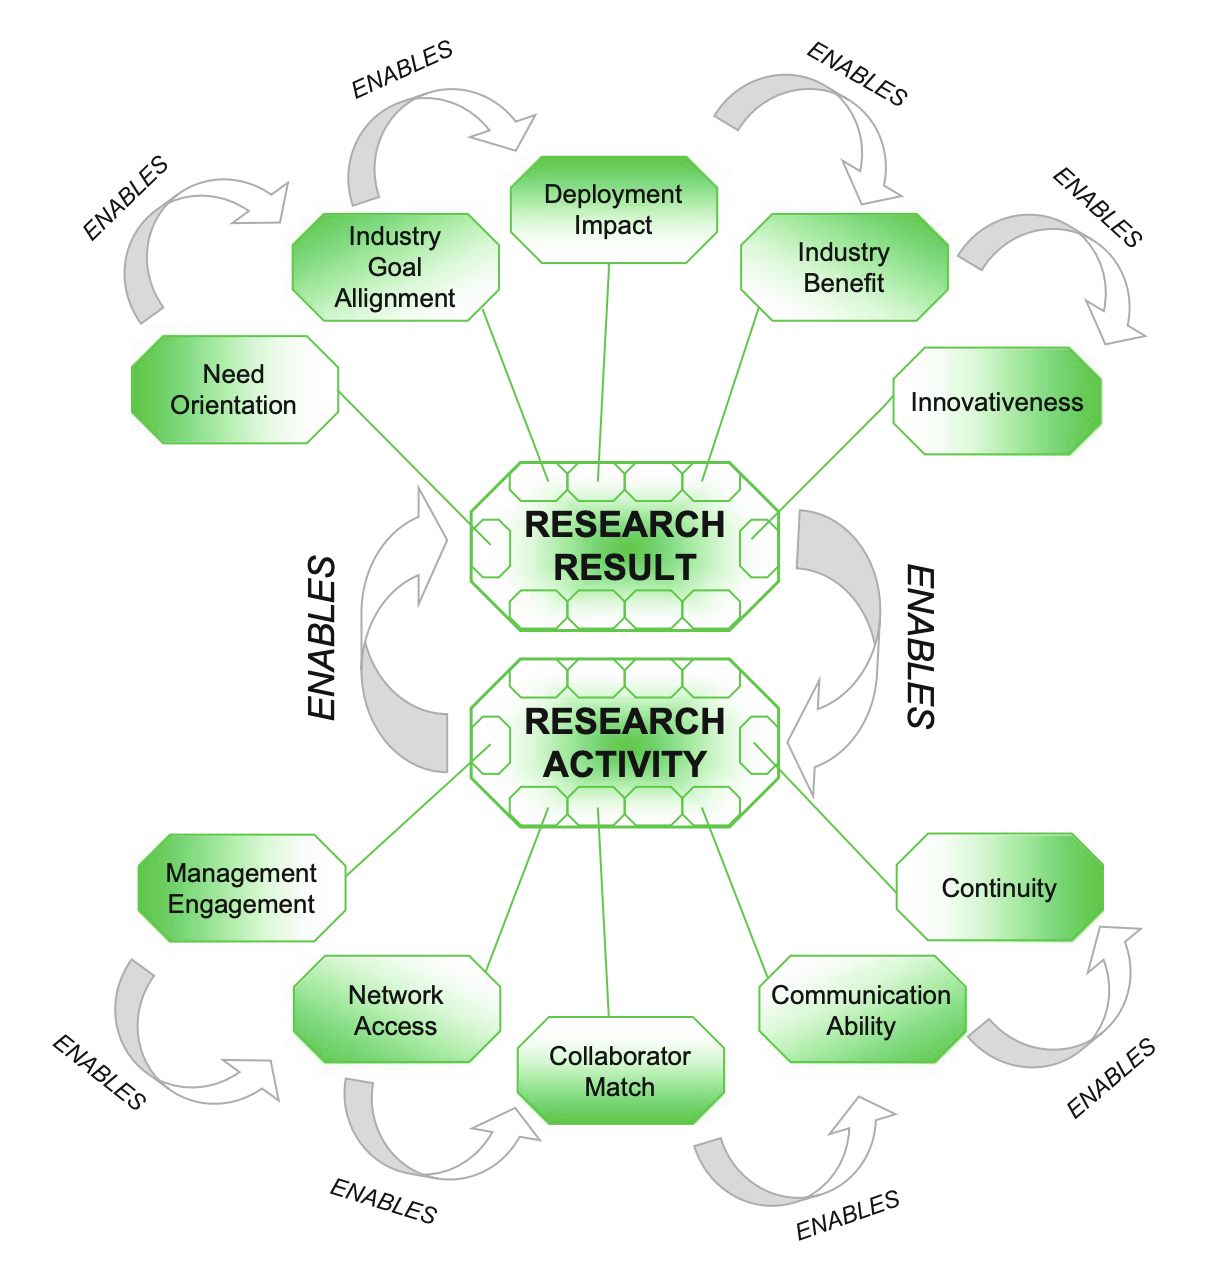
\includegraphics[width=.75\textwidth]{images/research.png}
% 	\end{center}
% 	\captionsetup{justification=centering}
% 	\caption{Success Factor Model for Academia-Industry Collaboration, Adapted from \protect\citeA[p. ~30]{bosch_2014}}
% 	\label{academia_industry}
% \end{figure}
    
    \subsection{Differences of Interpretation \& Implementation}
        \subsubsection{Viewpoint of Software Professionals}
        \begin{itemize}[noitemsep]
            \item How do software professionals interpret and implement CI/CD/CDE?
            \begin{itemize}
                \item \cite{atkinson_edwards_2018} \& \cite{stackify_2018}
            \end{itemize}
        \end{itemize}
        \subsubsection{Viewpoint of Academic Researchers}
        \begin{itemize}[noitemsep]
            \item How do academic researchers interpret and believe how CI/CD/CDE should be implemented?
            \begin{itemize}
                \item \cite{bosch_2014}, \cite{shahin_babar_zhu_2017}, \& \cite{stahl_2017}
            \end{itemize}
        \end{itemize}
        \subsubsection{Collaboration Effort}
        \begin{itemize}[noitemsep]
            \item What effort is there to bridge the phenomena of non-collaboration between developers and researchers?
            \begin{itemize}
                \item \cite{bosch_2014} \& \cite{stahl_2017}
            \end{itemize}
        \end{itemize}

    \subsection{Benefits of Continuous Integration, Delivery, \& Deployment}
        \subsubsection{Self-healing Systems}
        \begin{itemize}[noitemsep]
            \item What are the metrics and tools that software professionals use to mitigate having to manually fix software issues?
            \begin{itemize}
                \item \cite{bosch_2014}
            \end{itemize}
            \item How do these self-healing systems work?
            \begin{itemize}
                \item \cite{bosch_2014}
            \end{itemize}
        \end{itemize}
        \subsubsection{Risk Reduction}
        \begin{itemize}[noitemsep]
            \item How does continuous software engineering reduces risk in systems?
            \begin{itemize}
                \item \cite{atkinson_edwards_2018}, \cite{bosch_2014}, \cite{stackify_2018}, \& \cite{stahl_2017} \cite{stackify_2018}
            \end{itemize}
        \end{itemize}
        \subsubsection{Faster Release Cycles}
        \begin{itemize}[noitemsep]
            \item How are faster release cycles are achieved?
            \begin{itemize}
                \item \cite{atkinson_edwards_2018}, \cite{bosch_2014}, \cite{stackify_2018}, \& \cite{stahl_2017} \cite{stackify_2018}
            \end{itemize}
        \end{itemize}
        \subsubsection{Overall Cost Reduction}
        \begin{itemize}[noitemsep]
            \item Why will all of the above will reduce cost?
            \begin{itemize}
                \item \cite{atkinson_edwards_2018}, \cite{bosch_2014}, \cite{stackify_2018}, \& \cite{stahl_2017} \cite{stackify_2018}
            \end{itemize}
        \end{itemize}
        
    \subsection{Struggles of Traceability}
        \subsubsection{Importance}
        \begin{itemize}[noitemsep]
            \item What is the importance of traceability for the software engineering community?
            \begin{itemize}
                \item \cite{stahl_2017} \& \cite{stahl_hallen_bosch_2016}
            \end{itemize}
        \end{itemize}
        \subsubsection{Problem of Mapping}
        \begin{itemize}[noitemsep]
            \item What is the problem of mapping requirements to implemented code and the converse?
            \begin{itemize}
                \item \cite{stahl_2017} \& \cite{stahl_hallen_bosch_2016}
            \end{itemize}
        \end{itemize}
        \subsubsection{Eiffel Framework}
        \begin{itemize}[noitemsep]
            \item What is the proposed solution to address traceability issues in CI/CDE/CD environments?
            \begin{itemize}
                \item \cite{stahl_2017} \& \cite{stahl_hallen_bosch_2016}
            \end{itemize}
        \end{itemize}
        
    \subsection{Transition an Agile Environment}
        \subsubsection{The Effect of Organizational Change to Agile}
        \begin{itemize}[noitemsep]
            \item What are the problems that businesses face in attempt to switch to Agile practices?
            \begin{itemize}
                \item \cite{bosch_2014} \& \cite{meyer_2014}
            \end{itemize}
        \end{itemize}
        \subsubsection{Roles in Agile}
        \begin{itemize}[noitemsep]
            \item What are typical roles that each individual plays in an Agile environment?
            \begin{itemize}
                \item \cite{bosch_2014} \& \cite{meyer_2014}
            \end{itemize}
            \item Why do these roles exist?
            \begin{itemize}
                \item \cite{bosch_2014} \& \cite{meyer_2014}
            \end{itemize}
        \end{itemize}
        \subsubsection{Paradigm Shift in Leadership}
        \begin{itemize}[noitemsep]
            \item How has leadership changed as a result of Agile?
            \begin{itemize}
                \item \cite{bosch_2014}
            \end{itemize}
        \end{itemize}

\section{Conclusion}
    \subsection{Rephrase Thesis Statement}
    \subsection{Closing Statement}

\newpage
\section{Bibliography}
\nocite{*}
\bibliographystyle{apacite}
\bibliography{../bibliography}

\end{document}
